\section{A Replicated Tree Datatype}\label{sec:tree}

In \S~\ref{sec:datatypes} we gave an OpSet specification of a replicated object graph datatype.
In this model, every map or list object has a unique ID (namely, the ID of the $\mathsf{MakeMap}$ or $\mathsf{MakeList}$ operation that created it), and objects can reference each other using these IDs.

We now build upon this model, showing how to restrict the object graph so that it is always a tree.
A tree is a graph in which every vertex has exactly one parent (except for the root, which has no parent), and in which the parent relation has no cycles.
Tree data structures are useful in many applications: for example, file systems (consisting of directories and files) and XML or JSON documents are trees.
Branch nodes in this tree may be either maps or lists, and leaf nodes are primitive values (wrapped in a $\mathsf{MakeVal}$ operation).

\subsection{The Difficulty of a Move Operation}\label{sec:tree-difficult}

In applications that use tree-structured data, a frequently required operation is to \emph{move} a subtree to a new location within the tree.
For example:
\begin{itemize}
    \item In a filesystem, renaming a directory can be expressed as moving the directory node from the old name to the new name.
        Similarly, a directory may be moved to a new path.
    \item In vector graphics applications, several graphical objects may be grouped together as a logical unit.
        This operation can be expressed by creating a new branch node to represent the group, and then moving the individual objects to be children of that group node.
    \item In a to-do list application, users may use the order of items in the list to denote a priority order, and they may drag and drop items to change their relative order.
        Reordering items is equivalent to moving items to new locations within the list.
\end{itemize}

A move operation can be naively emulated by deleting the subtree from its old location and recreating it at the new location.
However, if two users perform this process concurrently, the resulting tree will contain two copies of the moved subtree, which would be undesirable in all of the application examples given above.
Thus, we require an \emph{atomic move} operation that does not create duplicate objects in case of concurrent moves.

\begin{figure}
\centering
\begin{tikzpicture}
  \tikzstyle{arrow}=[draw,-{Stealth[length=3.5mm]}]
  \node [rectangle,draw] (start) at (4,4) {
      \begin{tikzpicture}
      \node {$\mathsf{root}$} [level distance=9mm] child {node {$A$} child {node {$C$}}} child {node {$B$}};
      \end{tikzpicture}
  };
  \node [rectangle,draw] (left) at (1,2) {
      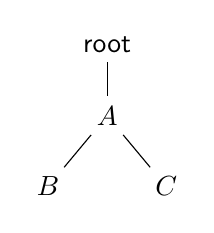
\begin{tikzpicture}
      \node {$\mathsf{root}$} [level distance=9mm] child {node {$A$} child {node {$B$}} child {node {$C$}}};
      \end{tikzpicture}
  };
  \node [rectangle,draw] (right) at (7,1.6) {
      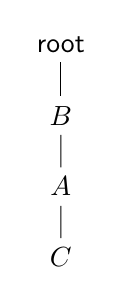
\begin{tikzpicture}
      \node {$\mathsf{root}$} [level distance=9mm] child {node {$B$} child {node {$A$} child {node {$C$}}}};
      \end{tikzpicture}
  };
  \node [rectangle,draw] (merge) at (4,-0.2) { ? };
  \node at (1.4,4.0) [text width=2.5cm,text centered] {Move $B$ to be a child of $A$};
  \node at (6.6,4.0) [text width=2.5cm,text centered] {Move $A$ to be a child of $B$};
  \draw [arrow] (start.west) -- (left);
  \draw [arrow] (start.east) -- (right);
  \draw [arrow] (left)  -- (merge.north west);
  \draw [arrow] (right) -- (merge.north east);
  \node at (4,0.6) {merge};
  %%%%%
  \node [rectangle,draw] at (9.9,4) {
      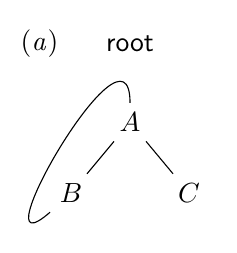
\begin{tikzpicture}
      \useasboundingbox (-1.3,-1.3) rectangle (1,1.2);
      \node at (-1.15,1.0) {(\emph{a})};
      \node at (0,1) {$\mathsf{root}$};
      \node (a1) {$A$} [level distance=9mm] child {node (b1) {$B$}} child {node {$C$}};
      \draw (b1.south west) .. controls (-2,-2) and (0,1.5) .. (a1.north);
      \end{tikzpicture}
  };
  \node [rectangle,draw] at (9.9,0.85) {
      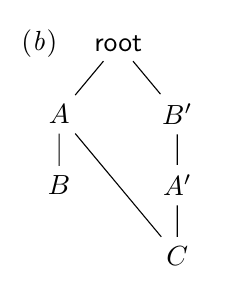
\begin{tikzpicture}
      \useasboundingbox (-1.15,-3.0) rectangle (1.15,0.2);
      \node at (-1.0,0.0) {(\emph{b})};
      \node {$\mathsf{root}$} [level distance=9mm] child {node (a2) {$A$} child {node {$B$}}} child {node {$B'$} child {node {$A'$} child {node (c2) {$C$}}}};
      \draw (a2) -- (c2);
      \end{tikzpicture}
  };
  \node [rectangle,draw] (start) at (12.5,4) {
      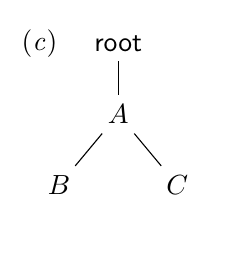
\begin{tikzpicture}
      \useasboundingbox (-1.15,-2.3) rectangle (1.15,0.2);
      \node at (-1.0,0.0) {(\emph{c})};
      \node {$\mathsf{root}$} [level distance=9mm] child {node {$A$} child {node {$B$}} child {node {$C$}}};
      \end{tikzpicture}
  };
  \node [rectangle,draw] (right) at (12.5,0.85) {
      \begin{tikzpicture}
      \useasboundingbox (-1.15,-3.0) rectangle (1.15,0.2);
      \node at (-1.0,0.0) {(\emph{d})};
      \node {$\mathsf{root}$} [level distance=9mm] child {node {$B$} child {node {$A$} child {node {$C$}}}};
      \end{tikzpicture}
  };
\end{tikzpicture}
\caption{Initially, $A$ and $B$ are siblings. $B$ is moved to be a child of $A$, while concurrently
$A$ is moved to be a child of $B$. Boxes (\emph{a}) to (\emph{d}) show possible outcomes of the merge.}\label{fig:concurrent-move}
\end{figure}

A more subtle kind of conflict is illustrated in Figure~\ref{fig:concurrent-move}.
Here, $B$ is moved to be a child of $A$, while concurrently $A$ is moved to be a child of $B$. 
If the CRDT does not take care to detect this situation, it may introduce a cycle in the merged result, as shown in Figure~\ref{fig:concurrent-move}(\emph{a});
this result is no longer a tree.
Handling such conflicting move operations is a challenging problem, and to our knowledge no existing implementation of a tree CRDT has found an adequate solution to this problem.

Several CRDT tree datatypes for XML \cite{Martin:2010ih,Nicolaescu:2015id} and JSON data \cite{Kleppmann:2016ve,Automerge,crjdt} have been developed, but to our knowledge, none of them define a move operation.
Tao et al.~\cite{Tao:2015gd} implemented a CRDT-based replicated filesystem, resolving concurrent moves with an approach illustrated in Figure~\ref{fig:concurrent-move}(\emph{b}): conflicting branch nodes (directories) are duplicated, and leaf nodes (files) may be referenced from multiple branch nodes.
Thus, Tao et al.'s data structure is strictly a DAG, not a tree.

Najafzadeh~\cite{Najafzadeh:2017vk,Najafzadeh:2018bw} also implemented a CRDT-based replicated filesystem, but chose a different approach: move operations must acquire a global lock before they can proceed, which ensures that conflicting concurrent move operations cannot occur in the first place.
This conservative approach rules out move conflicts, but the resulting datatype is not strictly a CRDT, since some operations require strongly consistent synchronisation.


\subsection{Specifying a Tree with Atomic Moves}\label{sec:tree-spec}

We now demonstrate the power of the OpSets approach by using it to define a tree CRDT with an anomaly-free atomic move operation.
Our specification rules out violations of the tree structure such as those in Figure~\ref{fig:concurrent-move}(\emph{a,b}), and concurrent moves do not duplicate tree nodes.
Moreover, our CRDT does not require any locks or global synchronisation.

When the OpSet contains conflicting move operations, our specification chooses one of them as the one that takes effect, and simply ignores the other conflicting operations.
Thus, in the example of Figure~\ref{fig:concurrent-move}, the merged outcome of the two conflicting move operations is either (\emph{c}) or (\emph{d}).
If two users concurrently move the same item to different locations, the move operation with the greater ID determines the item's final location.
However, in non-conflict situations, all concurrent move operations take effect.

We define a tree to be a restricted form of the object graph specified in \S~\ref{sec:datatypes}.
First, we require that there is a designated root object: assume that we have an operation ID $\mathsf{root}$ that is less than all other operation IDs (according to the total order on identifiers, introduced in \S~\ref{sec:system-model}).
Further assume that for any OpSet $O$ specifying a tree, we have either $(\mathsf{root},\, \mathsf{MakeList}) \in O$ or $(\mathsf{root},\, \mathsf{MakeMap}) \in O$, depending on whether the root node is a list or a map.
We define an object $x$ to be the \emph{parent} of an object $y$ if one of the values in $x$ is a reference to $y$.
The \emph{ancestor} relation is the transitive closure of the parent relation, defined using the element relation $E$:
\begin{align*}
    \mathsf{parent}(E,\, i) &=
    \begin{cases}
        \big\{ (\mathit{obj}, \mathit{val}) \mid \exists\,\mathit{id}, \mathit{key}.\;
            (\mathit{id}, \mathit{obj}, \mathit{key}, \mathit{val}) \in E \big\} & \text{if } i=1 \\
        \big\{ (x, z) \mid (x, y) \in \mathsf{parent}(E,\, i-1) \;\wedge\;
            (y, z) \in \mathsf{parent}(E,\, 1) \big\} & \text{if } i > 1
    \end{cases} \\[8pt]
    \mathsf{ancestor}(E) &= \bigcup_{i \;\geq\; 1} \mathsf{parent}(E,\, i)
\end{align*}

An object graph is a tree if the root has no parent, every non-root node has exactly one parent, and if the ancestor relation has no cycles.
We can redefine the operation interpretations from \S~\ref{sec:datatypes-interp} to preserve this tree invariant.
In fact, it is sufficient to redefine only the interpretation of $\mathsf{Assign}$, and to leave the interpretation of the other five operation types unchanged:
\begin{align*}
    \mathsf{interp}&\big[(E,\, L),\; (\mathit{id},\, \mathsf{Assign}(\mathit{obj}, \mathit{key}, \mathit{val}, \mathit{prev})) \big] \;=\\
    & \left\{
    \arraycolsep=0pt \def\arraystretch{1.5}
    \begin{array}{l}
        (E,\, L) \qquad \text{if } (\mathit{val},\, \mathit{obj}) \in \mathsf{ancestor}(E) \\[2pt]
        \Big( \big\{ (\mathit{id}', \mathit{obj}', \mathit{key}', \mathit{val}') \in E \mid
        \mathit{id}' \notin \mathit{prev} \wedge \mathit{val}' \neq \mathit{val} \big\} \;\cup\;
        \big\{ (\mathit{id}, \mathit{obj}, \mathit{key}, \mathit{val}) \big\},\; L \Big) \\
        \hphantom{(E,\, L)} \qquad \text{if } (\mathit{val},\, \mathit{obj}) \notin \mathsf{ancestor}(E)
    \end{array} \right.
\end{align*}

This definition differs in two ways from that in \S~\ref{sec:datatypes-interp}.
Firstly, the operation has no effect if $\mathit{val}$ is already an ancestor of the proposed parent $\mathit{obj}$, since the operation would otherwise introduce a cycle.
Secondly, any existing tuple in $E$ that references the same value $\mathit{val}$ is removed, preserving the invariant that every non-root node must have exactly one parent.

This interpretation of $\mathsf{Assign}$ performs an atomic move whenever $\mathit{val}$ is the ID of an existing object in the tree; in that case, it is moved from its existing position to the key $\mathit{key}$ in the object $\mathit{obj}$.
If $\mathit{val}$ does not currently exist in the tree (e.g.\ because it has just been created), the operation behaves like conventional assignment.
